Almost all processing tasks can display the input raw frames and the products in the so called "quality plots", which
can be inspected from the `Reduction Queue` window.
Those associated for the main product can be inspected by pressing the magnifying glass symbol at the right side of each dataset.
To inspect those associated to each individual job (if created), 

\begin{itemize}
 \item Expand the desired dataset by pressing the black arrow on its left. The list of jobs will appear with the associated status (COMPLETED, RUNNING, PENDING, MISSING, ABORTED, FAILED)
 \item Press the  magnifying glass symbol at the right side of the job you want to inspect. Only plots for completed jobs can be inspected.
\end{itemize}

 
\begin{figure}[h!]
\centering
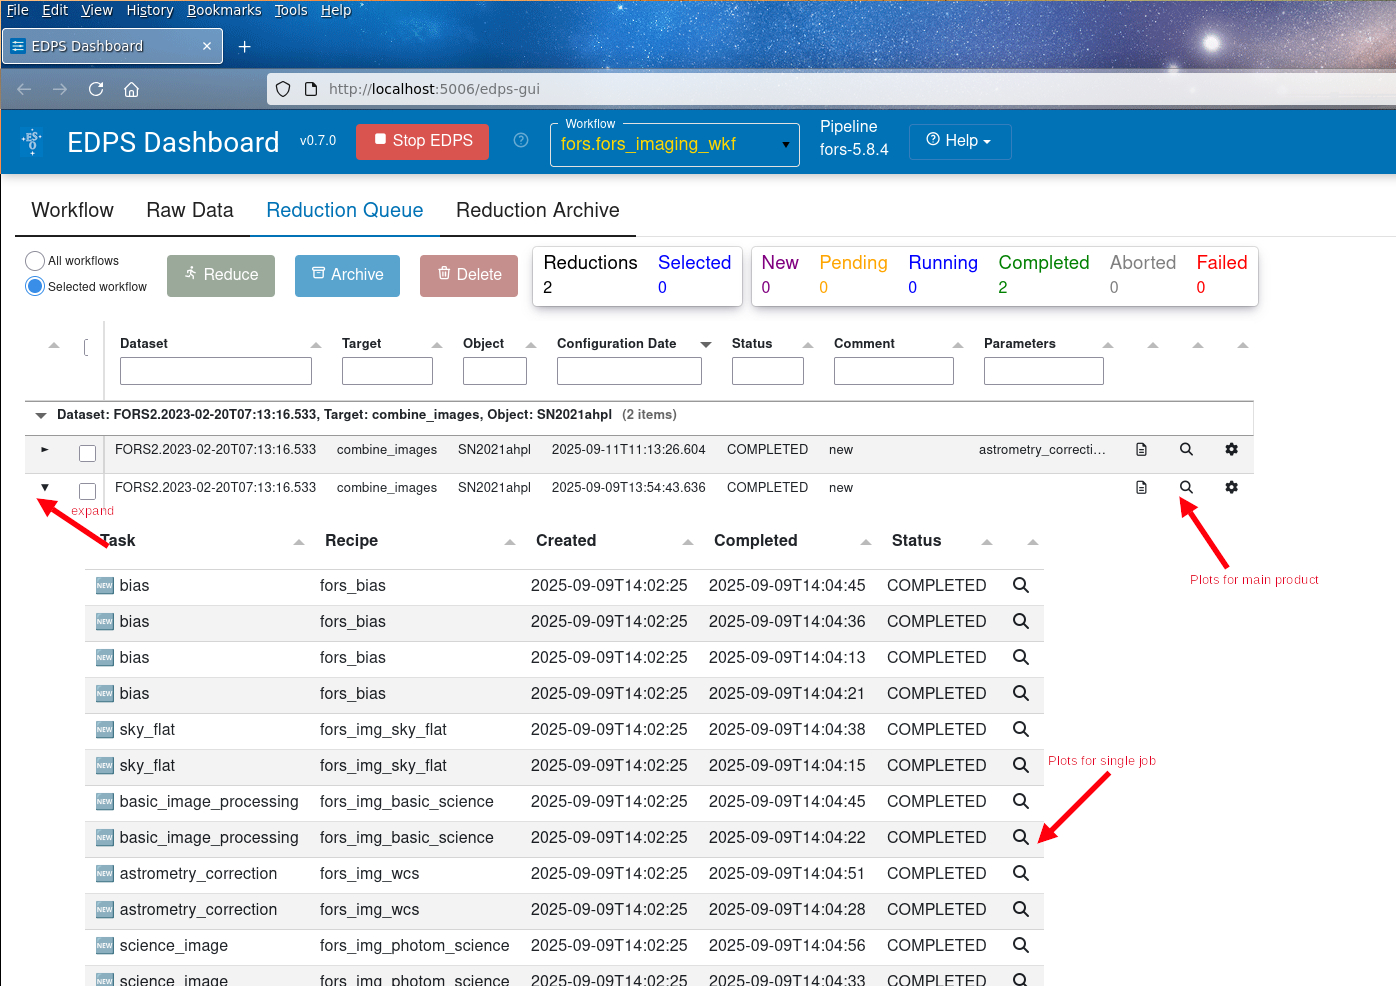
\includegraphics[width=0.9\textwidth]{../instrument_tutorial/figures/show_reports.jpg}
\caption{How to look for quality plots from the Reduction Queue tab.}
\label{fig:show_reports}
\end{figure}
